\subsection{Student~-Teacher Model: Basic Setup}
\label{sxn:SMOG_main-student_teacher}


\begin{figure}
  \centering
%  \includegraphics[width = 0.3\textwidth]{./img/perceptron.pdf}
  \begin{center}
  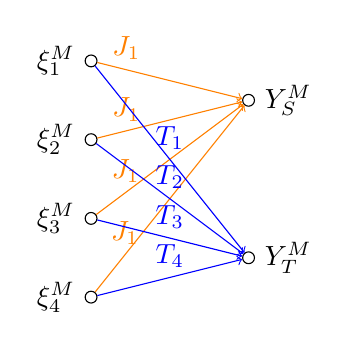
\begin{tikzpicture}
    \node[draw, circle, minimum size=0.15cm, inner sep=0.05cm] (A) at (0, 3) {};
    \node[draw, circle, minimum size=0.15cm, inner sep=0.05cm] (B) at (0, 2) {};
    \node[draw, circle, minimum size=0.15cm, inner sep=0.05cm] (C) at (0, 1) {};
    \node[draw, circle, minimum size=0.15cm, inner sep=0.05cm] (D) at (0, 0) {};

    \node[left] at (A.west) {$\xi_1^M$};
    \node[left] at (B.west) {$\xi_2^M$};
    \node[left] at (C.west) {$\xi_3^M$};
    \node[left] at (D.west) {$\xi_4^M$};

    \node[draw, circle, minimum size=0.15cm, inner sep=0.05cm] (Y) at (2, 2.5) {};
    \node[draw, circle, minimum size=0.15cm, inner sep=0.05cm] (Z) at (2, 0.5) {};

    \node[right] at (Y.east) {$Y_S^M$};
    \node[right] at (Z.east) {$Y_T^M$};
  
    % Arrows
    \draw[->, orange] (A) -- (Y) node[pos=0.2, above] {$J_1$};
    \draw[->, orange] (B) -- (Y) node[pos=0.2, above] {$J_1$};
    \draw[->, orange] (C) -- (Y) node[pos=0.2, above] {$J_1$};
    \draw[->, orange] (D) -- (Y) node[pos=0.2, above] {$J_1$};

    \draw[->, blue] (A) -- (Z) node[pos=0.5, above] {$T_1$};
    \draw[->, blue] (B) -- (Z) node[pos=0.5, above] {$T_2$};
    \draw[->, blue] (C) -- (Z) node[pos=0.5, above] {$T_3$};
    \draw[->, blue] (D) -- (Z) node[pos=0.5, above] {$T_4$};

  \end{tikzpicture}
  \end{center}
  \caption{Pictorial representation Student and Teacher Perceptrons.}
\end{figure}


In this subsection, we describe the basic setup of the \StudentTeacher model for computing the Average Empirical \Perceptron \GeneralizationError, $\AVGEMPGE$. 
We will do so for a simple Linear \Perceptron, when the students and teachers are modeled as vectors, as in traditional \SMOG, in the AA and at high-T.
%
For a simple \Perceptron, one can use the ST model to derive an expression for $\AVGSTGE$; and
one obtains a different expression depending on 
the type of \Perceptron (Linear or Boolean), 
the type of ensemble (microcanonical or canonical), 
the conditions on the learning (exact versus inexact), 
the type of approximation (\Annealed or \Quenched, \HighTemperature or Zero-Temperature), 
etc.~\cite{SST92}.
Here, we review the basic setup in order to give the reader a sense of the general approach and to give background for how we can use these results to formulate our \SETOL.

%%\nred{move this up:
%%Our goal here is to get a formal expression for the average \Student \Teacher (ST)
%%\GeneralizationError $\AVGSTGE$  as a \Student average, in the AA and at high-T, 
%%$\AVGSTGE=\THRMAVG{1-R}$ (\EQN~\ref{eqn:Eg_R2})
%%over ST overlap $R=\SVEC^{T}\TVEC$ between \Perceptron vectors,
%%and one that can be generalized from \Perceptron vectors into an expression
%%for the quality of single layer in NN weight matrices, and, importantly,
%%can then be be reformulated at as HCIZ integral in Section~\ref{sxn:matgen}.
%%}


\subsubsection{Test Error of the Teacher}

We start by describing how to obtain a simple formal expression for the empirical test error of the \Teacher \Perceptron.

Imagine a perceptron, called the \Teacher $(T)$, 
that maps some \emph{actual} (i.e., correlated) data
$\DATA\in\ADD$ to some known (binary) labels $\Yt$:
\begin{align}
 T:\DATA\rightarrow \MY^{T}_{\mu} ,
\end{align}
where the \Teacher \Perceptron is specified by some Energy function $E_{NN}$ (as in \EQN~\ref{eqn:dnn_energy}):
\begin{align}
\label{eqn:Eg_train}
\AVGEMPTE:= \frac{1}{N^{train}}\sum_{\mu=1}^{N^{train}}\mathcal{L}[\MY^{T}_{\mu},E_{NN}(\TVEC,\DATAtrain)]  .
\end{align}
We seek the true \GeneralizationError of the \Teacher, denoted  $\AVGGE^{T}$. 
Of course, this is usually unknowable; and so, in practice, one may try to estimate $\AVGGE^{T}$, e.g.,
by measuring the error of the \Teacher predictions on some test (or hold-out) set $(\DATA^{test}, \MY^{test})$.
We call this the \emph{\AverageGeneralizationError}, $\AVGEMPGE$.
Thus, we can write
\begin{align}
\label{eqn:Eg_test}
 \AVGGE^{T}\approx \AVGEMPGE:= \frac{1}{\Ntest}\sum_{\mu=1}^{\Ntest}\mathcal{L}[\MY^{T}_{\mu},E_{NN}(\TVEC,\DATAtest)] .
\end{align}
To measure the error, the loss function $\mathcal{L}$ may be a L1 $(\ell_1)$ or L2 $(\ell_2)$ loss;
whereas for training a model, it is usually something like a cross-entropy loss.
Here, we only consider the $\ell_2$ loss.

%Our goal is to develop a \SemiEmpirical theory for the matrix generalized form of $\AVGSTGE$,
%suitable for a single layer of a NN, and x denoted $\AVGNNGE$.


\subsubsection{Modeling Test Predictions with Student Perceptrons}

We now describe the how to estimate the \Teacher test \GeneralizationError, using a real-world, empirical distribution of Students.

In most theoretical analysis, one employs random i.i.d. data, not the actual training or test data (and certainly not real-world, strongly-correlated data) to estimate the average error, the \Typical error, or (say) trends in the average \GeneralizationError of a model $M$, i.e., $\AVGGE^{M}$.
We will estimate the average or \Typical \GeneralizationError for real system using real data  $(\DX)$ using techniques analogous to the techniques from \STATMECH.
%%, and in a practical setting.

To do so, imagine having another \Perceptron, 
called a \Student $(S)$ (with the same architecture as $T$, and acting on the same  
dataset $\DATA\in\ADD$), which tries to  reproduce the \Teacher predictions,
\begin{align}
S:\DATA\rightarrow \MY^{S}_{\mu}  ,
\end{align}
albeit imprecisely, and so $\MY^{S}_{\mu}\simeq \MY^{T}_{\mu}$. 

In this setup, we can write explicit expressions for the labels $\MY^{T}_{\mu}, \MY^{S}_{\mu}$
  in terms of the \Perceptron NN Energy (output / landscape) functions $E_{NN}$ (as in \EQN~\ref{eqn:dnn_energy})
\begin{align}
\nonumber
\Yt=E_{NN}(\TVEC, \DATA) \\ 
\Ys=E_{NN}(\SVEC,\DATA) ,
\end{align}
where the \Perceptron Energy $E_{NN}$, or output function,%
\footnote{Do not confuse the Energy/output function $E_{NN}$ with the energies $\mathbf{\Delta E}$  defined below to represent the ST error function(s).  We refer to outputs of $E_{NN}(\TVEC,\DATA )$, when applied to a data point $\DATA$, as energies because they are effectively un-normalized probabilities for the class outputs (for labels $\Ymu=1$ or $-1$).  }
is just the vector dot-product between the corresponding \Perceptron weight vector ($\TVEC$ or $\SVEC$)
and the (training or test) data vector $\DATA$:
\begin{align}
\label{eqn:ENN}
\nonumber
E_{NN}(\TVEC, \DATA)=h(\TVEC^{\top}\DATA) \\ 
E_{NN}(\SVEC, \DATA)=h(\SVEC^{\top}\DATA) ,
\end{align}
filtered through $h(x)$, some simple activation function (like a Heaviside step function $h(x)=\mbox{sgn}(x)$, or just the Identity $h(x)=x$).
For a Linear \Perceptron, we use an Identity activation, in which case we obtain
\begin{align}
\nonumber
\Yt=\TVEC^{\top}\DATA \\ 
\Ys=\SVEC^{\top}\DATA .
\end{align}
\michael{@charles: I just added that equation, so we can point to it explicitly later.}
\michaeladdressed{@charles: having T and S be superscripts there is confusing, especially later when these become vectors, subscripts would be better.}
\charles{All Transposes are with $\TR$ now, not $T$.   Lets discuss if still confusing.  Could make T, S script.}


To train a \Student \Perceptron $S$ that can learn how the \Teacher \Perceptron $T$ labels the training data $\DATAtrain$, 
one could break the data set into training $\DATAtrain$ and test $\DATAtest$ examples, 
train models on the training data (i.e., find the optimal model weights), 
and evaluate the model on the test data.
Then, the \Student learning task can therefore be written as in \EQN~(\ref{eqn:dnn_opt}) as the following optimization problem over the training data:
\begin{align}
\underset{\{\SVEC\}}{\argmin}\sum_{\mu=1}^{N^{train}}\mathcal{L}[E_{NN}(\SVEC,\DATA^{train}),E_{NN}(\TVEC,\DATAtrain)]   ,
\label{eqn:student-learning-task}
\end{align}
where the goal is to learn the \Student weight vector $\SVEC$, given the \Teacher vector $\TVEC$.
Notice that, at this step, the \Student $S$ and the \Teacher $T$ both depend explicitly on the specific choice of the training data $\DX_{train}$.  
That is, we could write $S[\DX^{train}], T[\DX^{train}]$.

Given such a student $\SVEC$, we could compute the \Teacher \GeneralizationError $\TGE^{T}$ by
replacing the test predictions in \EQN~\ref{eqn:Eg_test} with the student predictions
$y_{\mu}^{test}\rightarrow \Ys$, and then average directly over the test data $\DATAtest$
for all possible or available test examples.
%something like this below ?
%For a single student, in terms of the labels, and for $\mathcal{L}$ as an $\ell_2$ loss, 
%we can write the data-averaged ST error as
%\begin{equation} 
%\label{eqn:DE0}
%\langle\Delta \mathbf{E}_{\ell_2}(T,S)\langle_{\mathcal{D}} = \frac{1}{2} \sum_{\mu=1}^{N_{D}} (y_{t}^{\mu} - y_{s}^{\mu})^2  .
%\end{equation}
\michael{I'm a little confused. If deriving that is the point of the next subsubsection, we should give that equation very explicitly.  But I don't know if that is saying we should/will compute $\TGE^{T}$ or $\AVGEMPGE$ or what precisely.
}
In this way, we can model test predictions using one or more \Student \Perceptrons.



%\subsubsection{Empirical Training and Generalization Errors}
\subsubsection{Estimating the Average Empirical Generalization Error $(\AVGEMPGE)$}

If we have a very large number of suitable Students
(say, drawn from some random distribution), then we can try to estimate the 
\AverageGeneralizationError of the \Teacher, i.e., $\TGE^{T}\approx\AVGEMPGE$.
\michaeladdressed{That is a place where it is awkward to have an emph.  We are not defining either term, and I don't know where we define each term.  Is \EQN~\ref{eqn:emp_gen_error} the def.}
\michaeladdressed{Should ``If'' be ``it is''?  I'm not sure if this is a conditional, or basically the def.}
$\AVGEMPGE$ is given by an average loss, the average is 
over all possible Students $S$,  and then 
over all  $\Ntest$ test data points $\DATAtest\in\mathcal{D}$ 
%and (when the \Teacher is not fixed)
%over all equivalent Teachers (i.e., a uniform distribution of $\TVEC$ vectors that label the data in the same way):
%\michael{Why $p$ here and $N_D$ below, are they the same?  Also the data points are not $\mathcal{D}$, they are drawn from $\mathcal{D}$, correct?  In which case the sum below is either an integral over $\mathcal{D}$ which we empirically estimate, or is the empirical sum over the actual data?  (The basic idea is clear, just being more precise/pedantic.)}
%\charles{We discussed; please change if you like}
%\begin{align}
%\mathcal{E}_{t}^{emp}[\DX_{train}]=\frac{1}{Ntrain}\sum_{\mu=1}^{Ntrain}\left\langle\mathcal{L}[E_{NN}(\SVEC,\DATA_{train}),E_{NN}(\TVEC,\DATA_{train})]\right\rangle_{S}
%\label{eqn:emp_train_error}
%\end{align}
%and
\begin{align}
\AVGEMPGE[\DXtrain, \DXtest]=\frac{1}{\Ntest}\sum_{\mu=1}^{\Ntest}
\THRMAVG{\mathcal{L}[E_{NN}(\SVEC,\DATAtest),E_{NN}(\TVEC,\DATAtest)]} ,
\label{eqn:emp_gen_error}
\end{align}
where (ideally) $\Ntest$ is extremely large.
(As above, the loss function $\mathcal{L}$ may be an $\ell_1$ or an $\ell_2$ loss, etc.)
As in \EQN~\ref{eqn:thrmavg} (in Section~\ref{sxn:mathP}),
the brackets $\THRMAVG{\cdots}$ denote a \ThermalAverage of the Students vectors $\SVEC$.%
\footnote{This approach can be likened to the Bootstrap method~\cite{efron1993bootstrap} used for error estimation.  However, the Bootstrap method predominantly emphasizes variations in the input data $\NDX\in\mathcal{D}$, while in this context, we are essentially bootstrapping over the students $S$.}

%\michael{Is this for the optimal values of the parameters in the learning task \EQN~(\ref{eqn:student-learning-task})%?  Presumably not, since we are averaging? }
%\charles{Good question. We do not specify how the hyperparameters are selected.}

The empirical errors at this stage depend on the specific instantiation of the data  $\DX\in\ADD$.
Therefore, we may require resampling the training data and training an ensemble of models to compensate for anomalies in training data (bad labels, noise, etc.) that may cause the underlying model to overfit to the training data.
Theoretically, within \SMOG, this is equivalent to \emph{quenching} the system to the data (a term analogous to quickly cooling a physical system, frezing in any defects).
In contrast, when one \emph{anneals} a physical system, one heats up and cools it down slowly, and repeatedly, thereby removing any defects (of data anomalies for NNs, or material defects in a physical system).
%5We can write  $\AVGEMPGE[\DXtrain, \DXtest]$ explicitly in terms of the data.
%We now quench this estimate, averaging over the data disorder, or replicas $(\NDXItrain, \NDXItest)$, depicted as:
%Because of this, we dont have a complete estimate of the errors since there could be anomalies in the specific
%realization so the training or test data that we did not account for.
%To account for this, in the classic \STATMECH, one performs an additional \emph{quenched average}
%over
%\begin{align}
 % \AVGEMPGE[\DXtrain, \DXtest]\rightarrow\text{quench}\rightarrow\langle\AVGEMPGE[\NDXItrain, \NDXItest]\rangle_{\NDXI\in\mathcal{D}} \rightarrow \AVGEMPGE
%\end{align}
In \STATMECH, one can perform a so-called quenched average using a replica calculation,
effectively removing the dependence on test and/or training data
from the final estimate for $\AVGEMPGE$.
However, theoretical quenched result may differ significantly from the annealed case when the underlying model is unrealizable~\cite{SST92}. 
This may occur when the training data is very noisy and/or the model architecture is such that it can not correctly predict all the training labels.
In such cases, the model will always have some finite, non-zero Average \TrainingError, $\AVGTE > 0$,
even in the large-$N$ limit of infinite data.  In such a case, this indicates
a highly complex error landscape with many local minima separated by extremely high barriers,
and a slowing down of the dynamics.%
\footnote{In modern ML parlance, one might say the model can not be evaluated at interpolation, although 
in practice such a model might have a zero empirical \TrainingError since it may overfit the specific training data.}
\michael{This seems like important discussion, but it is related to what is going on in Section~\ref{sxn:SMOG_main-spin_glass}; I feel like we should have a minimalistic discussion of things like spin glasses in the main text, and then have a self-contained appendix that goes into it in more detail, since it gets in the way of getting to Section~\ref{sxn:SMOG_main-st_av} and Section~\ref{sxn:matgen}.  }
\charles{This is a minimal discussion.  }

While it is commonplace to train ensembles and/or use cross-validation when training small models (as the above discussion assumes),
this could be extremely expensive and impractical in modern ML, e.g., for very large models like LLMs~\cite{LLMS}.
For such massive NNs, one needs a theory that can detect anomalies in training directly from observations during and/or after training.
This is a hallmark of the \SETOL approach, and it distinguishes \SETOL from the classic \STATMECH approach.
\michael{MM TO DO: Probably move that to the intro.  That is an important par, too imp to be buried here.}
\charles{Not sure.  Intro is already long.  Maybe the conclusions}

%That said, it may be beneficial in practice to use subsamples of the training data to train the \Teacher and the Students
%when, say, the training data has mislabeled and/or noisy data.  With such bad data, the 
%results could be quite different after taking this additional step.
%Indeed, it is exactly these cases where the results differ theoretically as well as in practice.
%We will take a deeper look at such case of noisy data below.

%Importantly, we will not used the quenched form of $\mathcal{E}_{t}^{emp}$ because we will be able todetect
%anomalies in the training data directly by looking at the fitted \SemiEmpirical HT parameter $\alpha$.
